\section{The MitM Ontology for Computational Group Theory}\label{sec:cgt}
\begin{todolist}{MK@MP+DM: describe your work here}
\item talk about the levels (abstract, concrete subgroup theory, computational)
\item talk about alignments from the IFT to the CGT, how they work, building
  on~\cite{MueRoYuRa:abtafs17,MueGauKal:cacfms17} 
\end{todolist}

We chose computational group theory (CGT) to conduct a case study in creating
MitM ontologies. CGT is one of the oldest computational mathematics disciplines
and GAP already provides a strong template for the MitM ontology.

\subsection{Layers of Abstraction}


Our formalisation of CGT follows the template of its implementation in GAP, and
requires different levels of abstraction, currently \emph{abstract},
\emph{representation}, \emph{implementation}, and \emph{concrete}.
We expect this pattern to be applicable across computational algebra, possibly
with more levels of abstraction. Figure \ref{fig:cgtontology} shows the
levels and how the CGT ontology aligns with the GAP system dialect.

\documentclass{standalone}
\usepackage{amstext}
\usepackage{tikz}
\usetikzlibrary{shapes,arrows,fit}
\begin{document}
\providecommand{\mylabel}[1]{\begin{minipage}{2cm}\begin{center}#1\end{center}\end{minipage}}
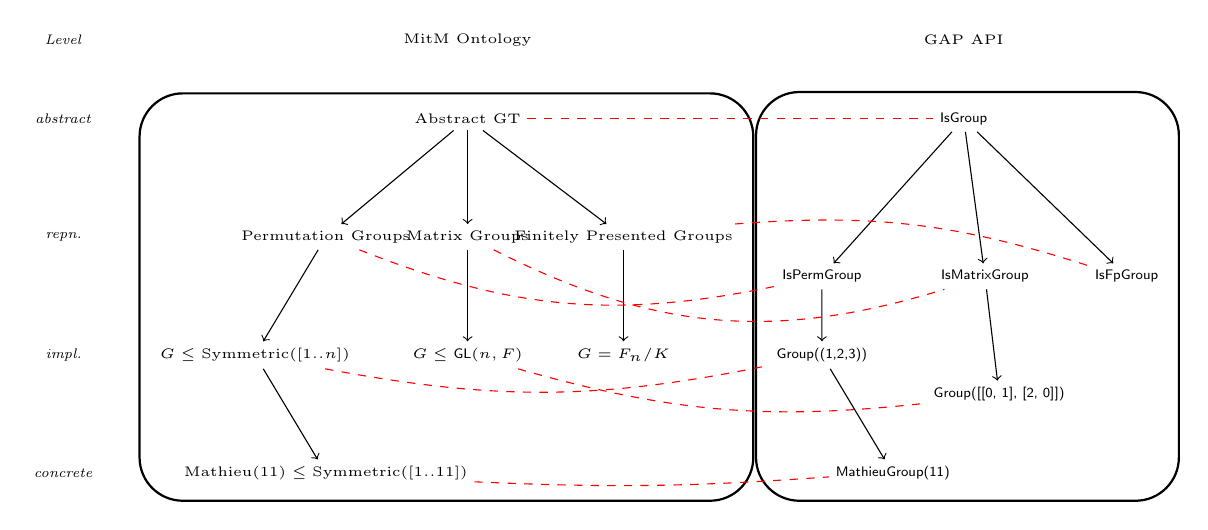
\begin{tikzpicture}[xscale=0.9]\tiny
\node (mitm) at (-2.7,8.5) {\emph{Level}}; 
\node (a) at (-2.7,7.5) {\emph{abstract}}; 
\node (b) at (-2.7,6) {\emph{repn.}}; 
\node (c) at (-2.7,4.5) {\emph{impl.}}; 
\node (d) at (-2.7,3) {\emph{concrete}}; 

\node (mitm) at (3,8.5) {MitM Ontology};

\node (grouptheory) at (3,7.5) {Abstract GT};
\node (permgrp) at (1,6) {\mylabel{Permutation Groups}};
\node (matgrp) at (3,6) {\mylabel{Matrix Groups}};
\node (finpresgrp) at (5.2,6) {\mylabel{Finitely Presented Groups}};
\draw[->] (grouptheory) -- (permgrp);
\draw[->] (grouptheory) -- (matgrp);
\draw[->] (grouptheory) -- (finpresgrp);

\node (symm) at (0,4.5) {$G\leq\text{Symmetric}([1..n])$};
\node (glnf) at (3,4.5) {$G\leq\textsf{GL}(n,F)$};
\node (fnk) at (5.2,4.5) {$G=F_n/K$};
\draw[->] (permgrp) -- (symm);
\draw[->] (matgrp) -- (glnf);
\draw[->] (finpresgrp) -- (fnk);

\node (mathieu) at (1,3) {$\text{Mathieu}(11)\leq\text{Symmetric}([1..11])$};
\draw[->] (symm) -- (mathieu);

 \node[draw,thick,fit=(grouptheory) (permgrp) (matgrp) (finpresgrp) (symm) (glnf) (fnk) (mathieu),
                   rounded corners=.55cm, inner sep=5pt] (mitmcloud) {};
                   
\node (gap) at (10,8.5) {GAP API};

\node (isgrp) at (10,7.5) {\textsf{IsGroup}};

\node (empty) at (10,3) {};
\node (ispermgrp) at (8,5.5) {\textsf{IsPermGroup}};
\node (ismatgrp) at (10.3,5.5) {\textsf{IsMatrixGroup}};
\node (isfpgrp) at (12.3,5.5) {\textsf{IsFpGroup}};
\draw[->] (isgrp) -- (ispermgrp);
\draw[->] (isgrp) -- (ismatgrp);
\draw[->] (isgrp) -- (isfpgrp);

\node (pgroup) at (8,4.5) { \textsf{Group((1,2,3))} };
\node (mgroup) at (10.5,4.0) { \textsf{Group([[0, 1], [2, 0]])} };
\node (cgroup) at (9,3)    { \textsf{MathieuGroup(11)} };

\draw[->] (ispermgrp) -- (pgroup);
\draw[->] (ismatgrp) -- (mgroup);
\draw[->] (pgroup) -- (cgroup);

 \node[draw,thick,fit=(isgrp) (ispermgrp) (ismatgrp) (isfpgrp) (empty) (pgroup) (mgroup) (cgroup),
                   rounded corners=.55cm, inner sep=5pt] (gapcloud) {};
                   
\draw[red,dashed] (grouptheory) -- (isgrp);
\draw[red,dashed] (permgrp) to[bend right=15] (ispermgrp);
\draw[red,dashed] (matgrp) to[bend right=20] (ismatgrp);
\draw[red,dashed] (finpresgrp) to[bend left=10] (isfpgrp);

\draw[red,dashed] (symm) to[bend right=10] (pgroup);
\draw[red,dashed] (glnf) to[bend right=10] (mgroup);
\draw[red,dashed] (mathieu) to[bend right=3] (cgroup);



%
%\node (Int) at (6,8.5) {Interfaces};
%
%\node (TT) at (4.9,3.5) {Type Theory};
%\node (ST) at (7.6,4.2) {Set Theory};
%\draw[<->,dotted] (TT) -- (ST);
%
%\node (Reals) at (4.7,4.8) {\textsf{Numbers}};
%\node (Nat) at (4.7,6) {$\mathbb N$};
%\draw[\arrowtipmono-\arrowtip] (Reals) -- (Nat);
%
%\node (FOrd) at (7.2,5.5) {Finite Ordinals};
%
%\node (PA) at (6,7) {Peano Axioms};
%\draw[<-] (FOrd) -- (PA);
%\draw[<-] (Nat) -- (PA);
%\draw[\arrowtipmono-\arrowtip] (ST) -- (FOrd);
%
% \node[draw,thick,fit=(ST) (Reals) (Nat) (FOrd) (PA) (TT),
%                   rounded corners=.55cm, inner sep=10pt] (PVScloud) {};
%
%\node (gap) at (11,8.5) {GAP API};
%
%\node (MNat) at (11,7) {\textsf{Nat}};
%\node (MOrd) at (11,3) {\textsf{Ordinals}};
%\draw[\arrowtipmono-\arrowtip] (MOrd) -- (MNat);
%
% \node[draw,thick,fit=(MNat) (MOrd),
%                   rounded corners=.55cm, inner sep=5pt] (PVScloud) {};
%
%\draw[red] (PVSfnd) -- (TT);
%\draw[red] (Mizfnd) -- (ST);
%\draw[red] (MOrd) -- (ST);
%\draw[red] (PVNat) -- (Nat);
%\draw[red] (PVnf) -- (Reals);
%\draw[red] (MNat) -- (FOrd);
%
%\draw[<->,dotted] (TT) -- (Reals);
%\draw[<->,dotted] (ST) -- (Reals);

\end{tikzpicture}
\end{document}

%%% Local Variables:
%%% mode: latex
%%% TeX-master: t
%%% End:

%  LocalWords:  providecommand mylabel tikzpicture mitm emph repn impl grouptheory matgrp
%  LocalWords:  permgrp finpresgrp symm leq glnf fnk draw,thick,fit mitmcloud isgrp FOrd
%  LocalWords:  ispermgrp ismatgrp isfpgrp gapcloud red,dashed mathbb arrowtipmono MNat
%  LocalWords:  arrowtip PVScloud MOrd PVSfnd Mizfnd PVnf

\medskip

At the abstract level, there is the theory of \emph{Groups}: the group axioms,
generating sets, homomorphisms, group actions, stabilisers, and orbits. This
also easily leads into definitions of centralisers\footnote{stabilisers of
elements under conjugation} and normalisers\footnote{stabilisers of subgroups under
conjugation}, stabiliser chains, Sylow-$p$ subgroups, Hall subroups, and many
other concepts. 

MMT also allows expressing that there are different equivalent definitions of a
concept: We defined group actions in two ways and used \emph{views} to express
their equivalence.

\smallskip

Abstract groups can be represented in many ways as concrete mathematical
objects suitable for computation: as groups of permutations, groups of matrices,
finitely presented groups, or using a polycyclic presentation.

Additionally, mathematicians often compute with canonical representatives of an
isomorphism class of groups: When a group theorist talks about the ``Dihedral
group of order 8'', they often have a particular representation in
mind, for example as a group that acts on the square by rotations
and reflections. In GAP this group would be represented as a group of
permutations, or by a polycyclic presentation.

Many representations arise naturally from \emph{group actions}: If we are
considering symmetry in a setting where we want to apply group theory, we start
with a group action.\ednote{MP@ALL: More concrete? More ``gripping''? I already
talked about the canonical example with the dihedral group}

The universal tool to bridge the gap between groups, representations and
canonical representatives are group homomorphisms, particularly isomorphisms,
which are used extensively in GAP. This is reflected in our approach.

\smallskip

At the lowest level there are implementation details: Permutation groups in GAP
are considered as finite subgroups of the group $S_{\mathbb{N}+}$, and defined by
providing a set of generating permutations. GAP then computes a stabiliser chain
for a group that was defined this way, and naturally considers the group to be a
subgroup of $S_{[1..n]}$, where $n$ is the largest point moved.

\smallskip

Building this part of the CGT MitM Ontology already posed a few challenges for
the MMT system, mostly to do with subtyping, since we needed to be able to talk
about all subgroups of a group, and all normal subgroups of a group. Quantifying
over these classes can lead to inconsistencies in the underlying type theory.
These challenges immediately translate into necessary
features in MMT, for example by introducing universe hierarchies.
\ednote{MP+FR+DM: Is this too gratuitous? Not concrete enough?}

\subsection{Alignments}

The initial alignments are currently produced by hand, but from some of the
initial alignments and the GAP API CDs we will be able to infer more alignments
automatically.

For example, the filter \texttt{IsGroup} is aligned with \texttt{Group}, and the
filter \texttt{IsPermGroup} is aligned with \texttt{Subgroup SymmetricGroup
  [1..n]}.
\ednote{MP: Need to be more concrete here, in particular we should maybe
  describe how GAP's notion of an action homomorphism translates through this?
  Also is this even correct?}

We formalised the theory of symmetric groups of a set; in GAP permutation groups
are represented as subgroups (with finite support) of the symmetric group of
$\mathbb{N}+$, and often one concretely has an isomorphism between the group one
is interested in and a subgroup of $S_{\mathbb{N}+}$, for example
via a group action.

\texttt{SylowSubgroup}s are more difficult: They are special groups in their
own right, namely groups whose size is a prime-power, but we also want them
to be identified with a certain subgroup of the group we are working
with.\ednote{MP: While I believe this to be an excellent additional example
  for MMT formalisation, this could be going too far for this paper}

\ednote{MP@ALL: We might want to be a bit careful/mention implementations of group
  theory for example in COQ where they did the Odd-Order-Proof?}
%%% Local Variables:
%%% mode: latex
%%% TeX-master: "paper"
%%% End:

%  LocalWords:  sec:cgt MueRoYuRa:abtafs17,MueGauKal:cacfms17 emph Sylow subroups medskip
%  LocalWords:  mathbb fig:cgtontology alignmentimg smallskip subtyping
